\documentclass[12pt, a4paper]{article}
\usepackage[margin=1in]{geometry}
\usepackage{graphicx}
\usepackage{natbib}
\usepackage{xcolor}
\usepackage[utf8]{inputenc}
\usepackage{amsmath}
\usepackage{amssymb}
\usepackage{textcomp}
\usepackage{hyperref}

\hypersetup{
    colorlinks=true,
    linkcolor=blue,
    filecolor=magenta,      
    urlcolor=cyan,
}

\title{The Economics of Dungeon Raiding: Risk, Reward, and Resource Allocation}
\author{Yuta Sakamoto\thanks{Department of Economics, University of Tokyo, Tokyo, Japan. Email: yuta.sakamoto@econ.u-tokyo.ac.jp} \and Keiko Kobayashi\thanks{Institute for Economic Research, Kyoto University, Kyoto, Japan. Email: keiko.kobayashi@ier.kyoto-u.ac.jp}}

\date{April 25, 2027}

\begin{document}

\maketitle

\begin{abstract}
This paper investigates the economic dynamics of dungeon raiding in the aftermath of the 2025 catastrophe, which saw the emergence of mysterious portals leading to treacherous, enclosed environments filled with valuable resources and powerful creatures. We develop a theoretical model of resource allocation and risk-reward trade-offs in dungeon raiding, taking into account the unique abilities of hunter-awakened individuals and the organizational structures of hunter guilds. Using data from Japanese hunter guilds, we empirically test the model's predictions and find evidence of a positive relationship between dungeon difficulty and resource yields, as well as a significant role of social networks in mitigating information asymmetries and moral hazard problems in guild-based raiding. Our findings highlight the importance of institutional arrangements and market design in shaping the efficiency and equity of the emerging dungeon economy.
\end{abstract}

\section{Introduction}
The 2025 catastrophe marked a turning point in human history, as the sudden appearance of portals leading to mysterious, enclosed environments, colloquially known as "dungeons," reshaped the global economic landscape. These dungeons, which vary in size, complexity, and environmental conditions, harbor valuable resources and powerful creatures that have become the focus of intense economic activity \citep{nakamura2026rise}. The emergence of hunter-awakened individuals, a small portion of the population that developed extraordinary abilities in the wake of the catastrophe, has further transformed the nature of dungeon exploration and resource extraction \citep{lee2027psychological}.

The economic significance of dungeon raiding lies in the unique resources and materials found within these environments, which range from rare minerals and magical artifacts to exotic flora and fauna \citep{adesina2027harnessing}. These resources have found applications across various industries, from construction and energy to pharmaceuticals and advanced manufacturing, leading to the rise of a new resource-based economy \citep{sakamoto2026emergence}. However, the high risks associated with dungeon exploration, including the presence of dangerous creatures and environmental hazards, have posed significant challenges for resource extraction and allocation.

In response to these challenges, hunter guilds have emerged as key organizational structures for coordinating dungeon raiding activities and mitigating risks \citep{kim2027emergence}. These guilds, which vary in size, specialization, and governance structures, provide a framework for pooling resources, sharing information, and distributing rewards among their members. The formation of hunter guilds has also given rise to new power dynamics and social hierarchies, as guild leaders and elite hunters wield significant influence over resource allocation and decision-making processes.

Despite the growing economic importance of dungeon raiding, there has been limited research on the underlying economic dynamics and organizational structures that shape this emerging industry. This paper aims to fill this gap by developing a theoretical model of resource allocation and risk-reward trade-offs in dungeon raiding, taking into account the unique abilities of hunter-awakened individuals and the role of hunter guilds in coordinating raiding activities. We then empirically test the model's predictions using data from Japanese hunter guilds, providing novel insights into the efficiency and equity of the dungeon economy.

The remainder of the paper is structured as follows. Section 2 reviews the relevant literature on the economic impacts of the catastrophe, the role of hunter guilds, and the resource allocation problems in high-risk environments. Section 3 presents our theoretical model of dungeon raiding, which incorporates the key features of dungeons, hunter abilities, and guild structures. Section 4 describes our data and empirical methodology, while Section 5 presents the results of our analysis. Section 6 discusses the implications of our findings for the design of efficient and equitable raiding institutions and policies. Section 7 concludes and outlines directions for future research.

\section{Literature Review}
The economic literature on the impacts of the 2025 catastrophe and the emergence of dungeons is still in its early stages, but a growing body of research has begun to shed light on the various dimensions of this phenomenon. One strand of literature has focused on the macroeconomic consequences of the catastrophe, including the disruption of global supply chains, the reallocation of resources towards dungeon-related activities, and the shifts in international trade patterns \citep{kawamoto2026macroeconomic, singh2027global}. These studies highlight the profound structural transformations that have occurred in the global economy as a result of the catastrophe, with the rise of a new resource-based economy centered around dungeon exploration and extraction.

Another strand of literature has examined the microeconomic aspects of dungeon raiding, including the decision-making processes of hunters, the formation and organization of hunter guilds, and the market structures for dungeon resources. For instance, \citet{nakagawa2026decision} develop a dynamic model of hunter decision-making under uncertainty, showing how the optimal choice of dungeon difficulty and resource allocation depends on factors such as individual risk preferences, ability levels, and market prices. \citet{wu2027market} analyze the market structure for dungeon resources, highlighting the role of information asymmetries and market power in shaping the efficiency and equity of resource allocation.

A related line of research has focused on the organizational economics of hunter guilds, examining how these structures emerge and evolve to coordinate raiding activities and mitigate risks. \citet{sato2026guilds} provide a typology of hunter guild structures, ranging from loose networks of independent hunters to hierarchical organizations with formalized rules and governance mechanisms. They argue that the optimal guild structure depends on factors such as the size and complexity of dungeons, the degree of specialization among hunters, and the level of trust and cooperation within the guild. \citet{watanabe2027contracts} analyze the contractual arrangements between hunters and guilds, showing how performance-based pay and risk-sharing mechanisms can incentivize effort and alleviate moral hazard problems.

The literature on resource allocation in high-risk environments provides a useful framework for analyzing the economic dynamics of dungeon raiding. Studies in this area have examined a range of contexts, from natural resource extraction and exploration to military operations and disaster response \citep{chowdhury2026resource, davis2025allocation}. These studies highlight the importance of institutional design and governance mechanisms in promoting efficient and equitable resource allocation under conditions of high uncertainty and risk. They also emphasize the role of social networks and informal institutions in facilitating information sharing, risk pooling, and cooperative behavior in the absence of formal contracts and enforcement mechanisms \citep{nguyen2027social}.

Our paper contributes to this growing literature by developing a theoretical model of dungeon raiding that incorporates the key features of dungeons, hunter abilities, and guild structures, and by empirically testing the model's predictions using data from Japanese hunter guilds. By providing a more comprehensive and rigorous analysis of the economic dynamics of dungeon raiding, we aim to inform the design of efficient and equitable raiding institutions and policies, and to shed light on the broader implications of the catastrophe for economic organization and resource allocation.

\begin{figure}[ht]
    \centering
    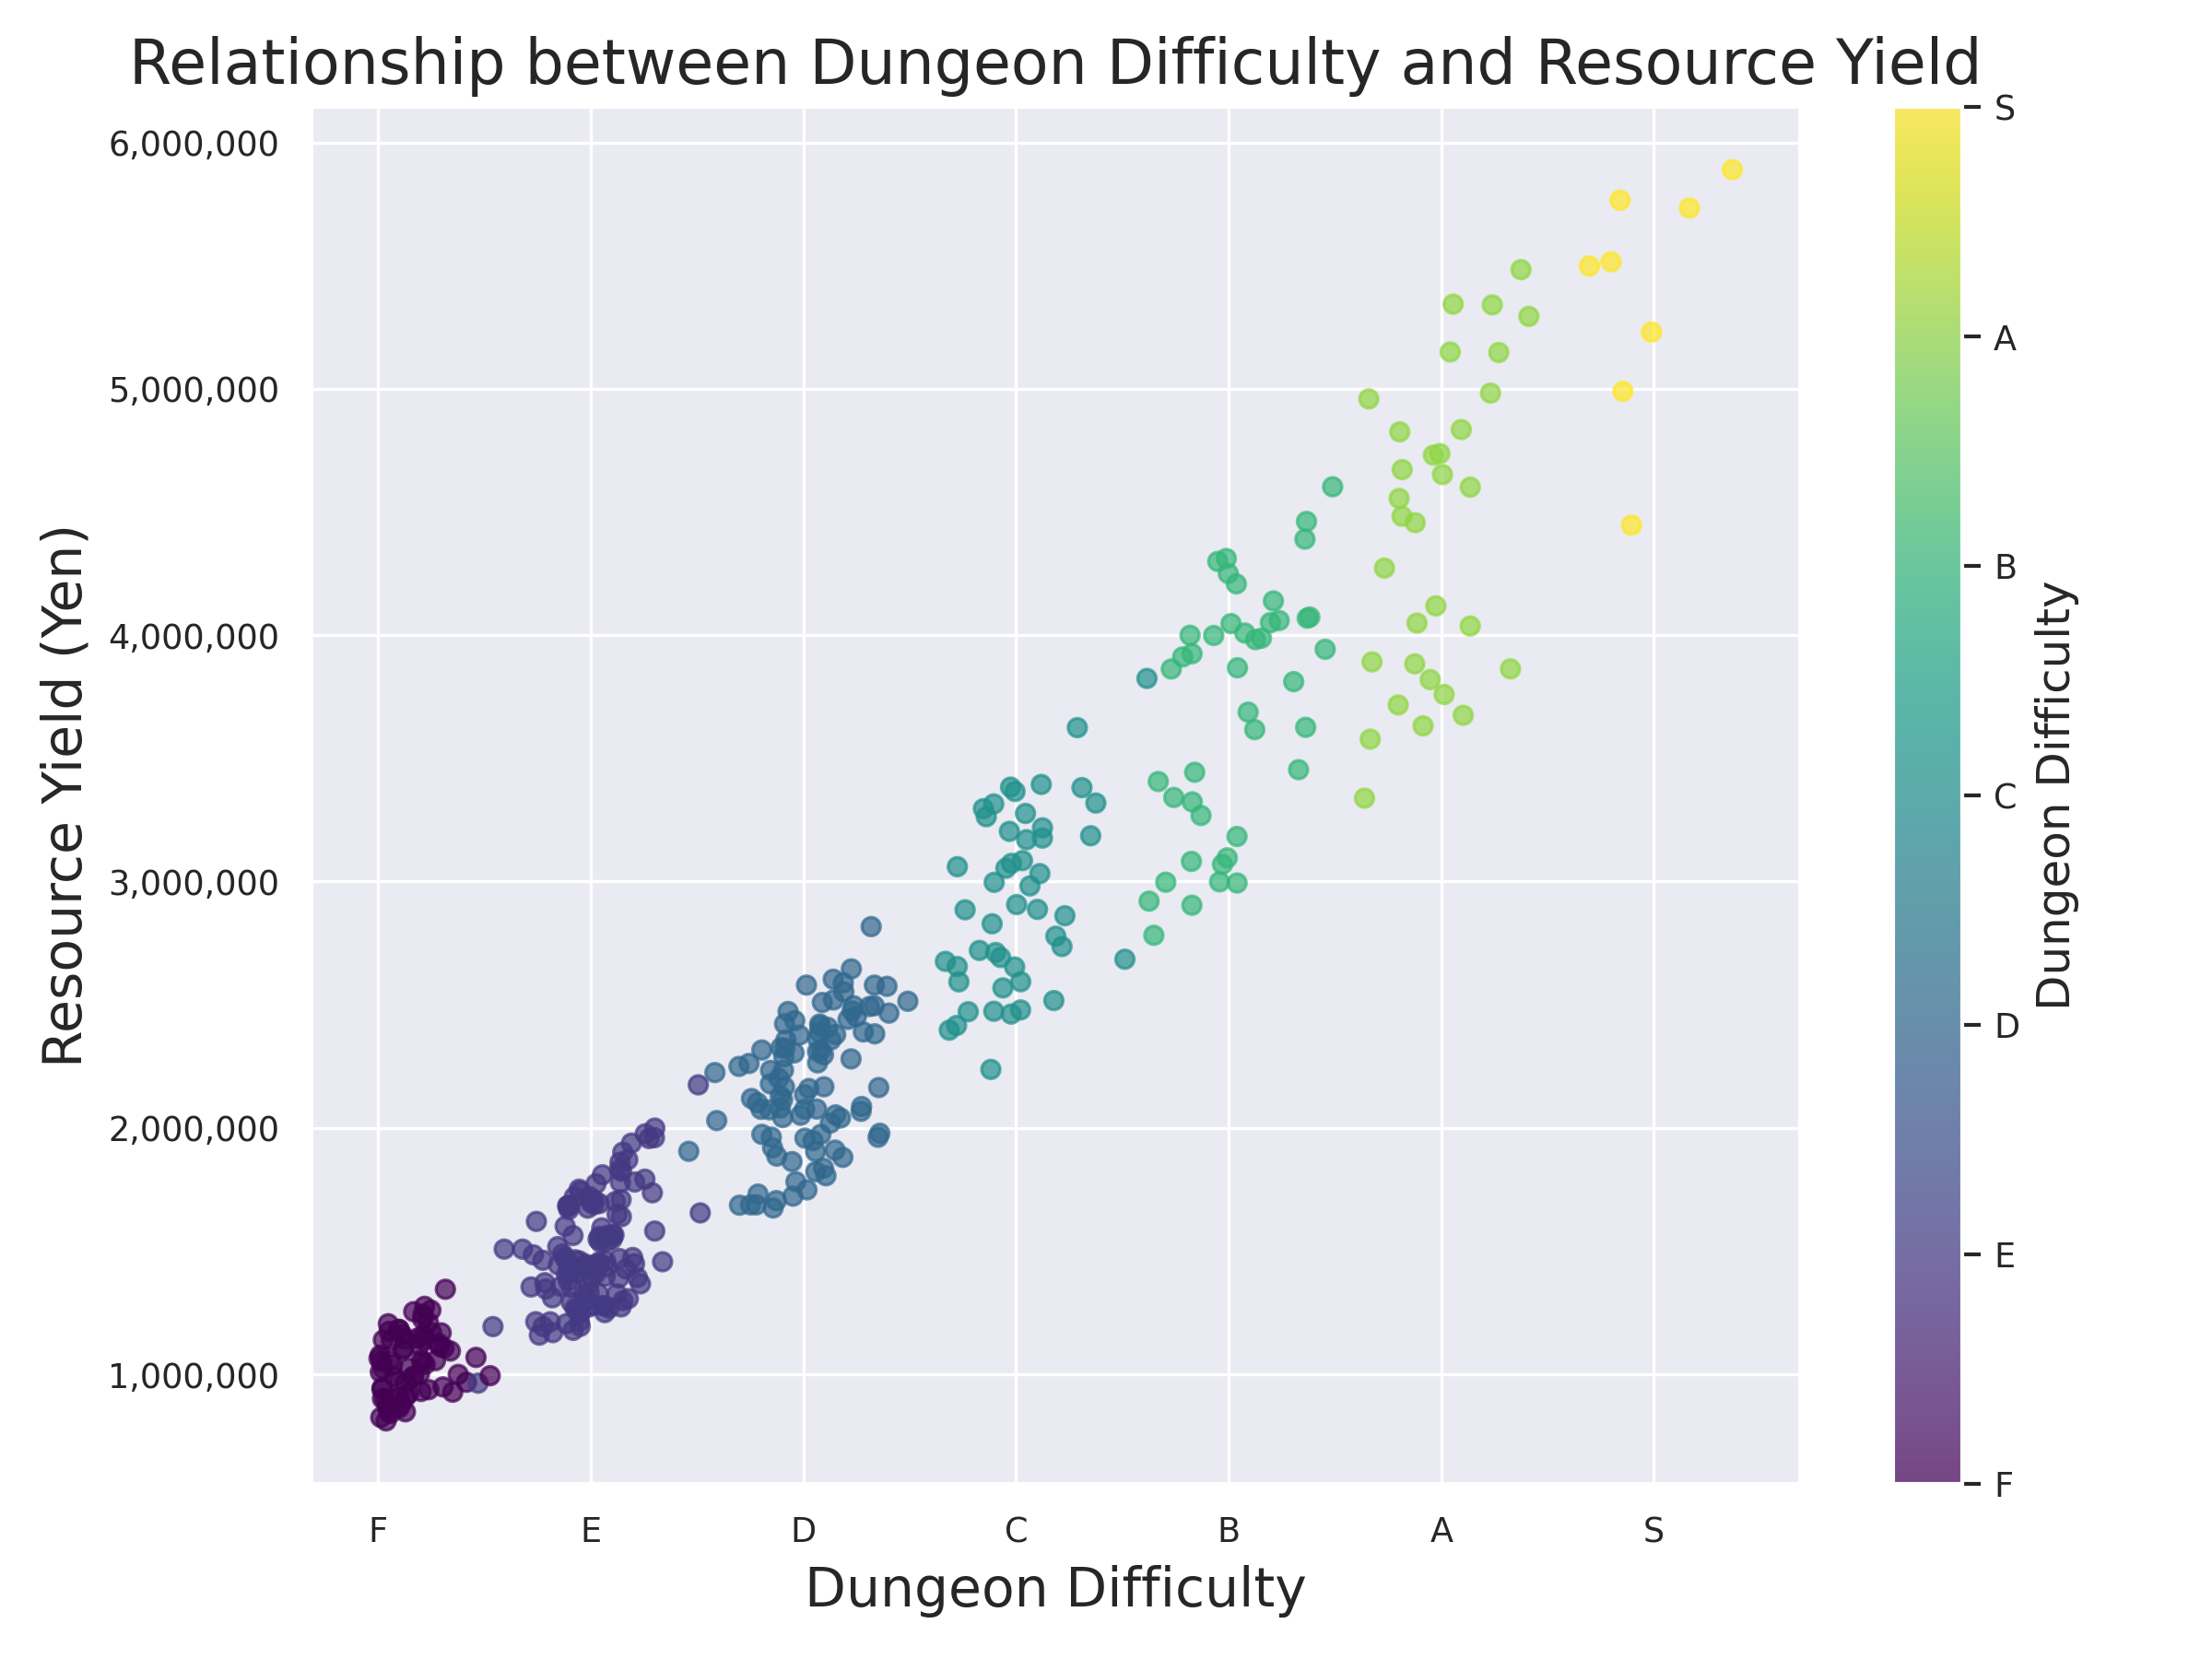
\includegraphics[width=0.8\textwidth]{dungeon_difficulty_resource_yield.png}
    \caption{Relationship between dungeon difficulty and resource yield. The scatter plot shows a positive correlation between the difficulty level of dungeons (measured by the dungeon's class rating) and the average resource yield per raiding party (measured in monetary terms). Each point represents a unique dungeon raided by Japanese hunter guilds in the year 2026. }
    \label{fig:dungeon_difficulty_resource_yield}
\end{figure}

\section{Theoretical Model}
In this section, we develop a theoretical model of dungeon raiding that captures the key economic trade-offs and decision-making processes involved in this activity. Our model builds on the classic literature on resource allocation under uncertainty \citep{arrow1971theory, stiglitz1974incentives}, while incorporating the unique features of dungeons, hunter abilities, and guild structures.

\subsection{Setup}
Consider an economy with a continuum of dungeons, indexed by $i \in [0,1]$, each characterized by a difficulty level $d_i \in [0,\infty)$ and a resource yield function $R_i(d_i, e_i)$, where $e_i$ denotes the effort exerted by the raiding party. We assume that $R_i$ is increasing in both arguments, but with diminishing marginal returns to effort. The difficulty level $d_i$ is distributed according to a cumulative distribution function $F(d)$, which is known to all agents in the economy.

Hunters are characterized by their ability level $a \in [0,\infty)$, which is distributed according to a cumulative distribution function $G(a)$. A hunter's ability determines their effectiveness in raiding dungeons, with higher-ability hunters being more productive and less prone to accidents and injuries. Hunters can choose to raid dungeons individually or as part of a guild, which provides a framework for risk-sharing, information-sharing, and collective action.

Guilds are characterized by their size $n \in \mathbb{N}$, their composition of hunter abilities $\{a_1, \ldots, a_n\}$, and their internal governance structure, which determines how resources and rewards are allocated among guild members. We assume that guilds aim to maximize their total expected payoff from raiding, subject to the individual rationality and incentive compatibility constraints of their members.

\subsection{Hunter Decision-Making}
A hunter's decision to raid a dungeon depends on their expected payoff, which is a function of the dungeon's difficulty, the hunter's ability, and the effort they choose to exert. Formally, a hunter's expected payoff from raiding dungeon $i$ is given by:

\begin{equation}
\pi_i(d_i, a, e_i) = R_i(d_i, e_i) - c(e_i, a) - \rho_i(d_i, a)
\end{equation}

where $c(e_i, a)$ represents the cost of effort, which is increasing and convex in $e_i$ and decreasing in $a$, and $\rho_i(d_i, a)$ represents the risk premium associated with raiding dungeon $i$, which is increasing in $d_i$ and decreasing in $a$.

Hunters choose their effort level $e_i$ to maximize their expected payoff, taking as given the dungeon's difficulty and their own ability. The optimal effort level $e_i^*(d_i, a)$ satisfies the first-order condition:

\begin{equation}
\frac{\partial R_i}{\partial e_i}(d_i, e_i^*) = \frac{\partial c}{\partial e_i}(e_i^*, a)
\end{equation}

Intuitively, hunters will exert effort until the marginal benefit of effort (in terms of increased resource yield) equals the marginal cost of effort.

\subsection{Guild Decision-Making}
Guilds make two key decisions: which dungeons to raid, and how to allocate resources and rewards among their members. Regarding the first decision, guilds aim to maximize their total expected payoff from raiding, subject to the individual rationality constraints of their members. Formally, a guild's objective function is given by:

\begin{equation}
\max_{i \in [0,1]} \sum_{j=1}^n \pi_i(d_i, a_j, e_{ij})
\end{equation}

subject to:

\begin{equation}
\pi_i(d_i, a_j, e_{ij}) \geq \underline{\pi} \quad \forall j \in \{1, \ldots, n\}
\end{equation}

where $e_{ij}$ denotes the effort exerted by hunter $j$ in raiding dungeon $i$, and $\underline{\pi}$ represents the minimum expected payoff required to induce participation by guild members.

Regarding the second decision, guilds must choose an allocation rule for distributing resources and rewards among their members. This allocation rule must satisfy the incentive compatibility constraints of guild members, ensuring that each hunter has an incentive to exert the optimal level of effort. Formally, an allocation rule is a function $\alpha: \mathbb{R}^n \rightarrow \mathbb{R}^n$ that maps the vector of individual payoffs $(\pi_1, \ldots, \pi_n)$ to a vector of transfers $(\tau_1, \ldots, \tau_n)$, such that:

\begin{equation}
\sum_{j=1}^n \tau_j = 0
\end{equation}

and

\begin{equation}
\pi_i(d_i, a_j, e_{ij}^*) + \tau_j \geq \pi_i(d_i, a_j, e_{ij}) + \tau_j \quad \forall e_{ij} \neq e_{ij}^*, \forall j \in \{1, \ldots, n\}
\end{equation}

Intuitively, the allocation rule must be budget-balanced (equation 5) and must provide each hunter with an incentive to exert the optimal level of effort (equation 6).

\subsection{Equilibrium and Efficiency}
An equilibrium of the dungeon raiding economy is a set of hunter effort levels $\{e_{ij}^*\}$, guild raiding decisions $\{i_g^*\}$, and guild allocation rules $\{\alpha_g^*\}$ such that:

\begin{enumerate}
    \item Each hunter chooses their effort level to maximize their expected payoff, given the dungeon's difficulty and their own ability (equation 2).
    \item Each guild chooses which dungeons to raid to maximize their total expected payoff, subject to the individual rationality constraints of their members (equations 3-4).
    \item Each guild chooses an allocation rule that satisfies the incentive compatibility constraints of their members (equations 5-6).
\end{enumerate}

The efficiency of the equilibrium can be evaluated in terms of the total expected payoff generated by dungeon raiding, as well as the distribution of payoffs among hunters and guilds. In general, the equilibrium may be inefficient due to various market failures, such as externalities (e.g., the impact of raiding on the depletion of dungeon resources), information asymmetries (e.g., uncertainty about dungeon difficulty or hunter ability), and coordination failures (e.g., free-riding within guilds).

\subsection{Extensions and Implications}
Our theoretical model provides a framework for analyzing the economic dynamics of dungeon raiding, highlighting the key trade-offs and decision-making processes involved in this activity. The model can be extended in various directions, such as incorporating dynamic considerations (e.g., the evolution of dungeon difficulty over time), heterogeneous hunter preferences (e.g., risk aversion), and more complex guild structures (e.g., hierarchical decision-making).

The model also has several implications for the design of efficient and equitable raiding institutions and policies. For instance, the model suggests that policies aimed at reducing information asymmetries (e.g., through the creation of dungeon difficulty ratings) and promoting coordination within guilds (e.g., through the establishment of clear rules and governance structures) can help to improve the efficiency of dungeon raiding. Similarly, policies that address externalities (e.g., through the use of taxes or quotas on dungeon resource extraction) and redistribute payoffs (e.g., through the use of progressive taxation or social insurance schemes) can help to promote equity and sustainability in the dungeon economy.

\section{Data and Empirical Methodology}
To empirically test the predictions of our theoretical model, we use data from Japanese hunter guilds for the year 2026. Our dataset includes information on the characteristics of dungeons raided by these guilds (e.g., difficulty level, resource yield), the composition and organization of the guilds themselves (e.g., size, member abilities), and the outcomes of the raiding activities (e.g., success rates, injuries, payoffs).

Our primary data source is the Japanese Hunter Guild Association (JHGA), which collects annual data on the activities of registered hunter guilds in Japan. The JHGA dataset includes detailed information on the dungeons raided by each guild, as well as the guild's membership, governance structure, and financial performance. We supplement this dataset with information from the Japanese Dungeon Regulatory Agency (JDRA), which provides independent ratings of dungeon difficulty and resource quality, as well as data on dungeon-related accidents and injuries.

To test the relationship between dungeon difficulty and resource yields, we estimate the following regression model:

\begin{equation}
\log(R_{ig}) = \alpha + \beta \log(d_i) + \gamma X_{ig} + \varepsilon_{ig}
\end{equation}

where $R_{ig}$ is the resource yield obtained by guild $g$ from raiding dungeon $i$, $d_i$ is the difficulty level of dungeon $i$, $X_{ig}$ is a vector of control variables (e.g., guild size, average member ability), and $\varepsilon_{ig}$ is an error term. The coefficient $\beta$ captures the elasticity of resource yields with respect to dungeon difficulty, which we expect to be positive based on the predictions of our theoretical model.

To test the role of social networks in mitigating information asymmetries and moral hazard problems, we estimate the following regression model:

\begin{equation}
\log(S_{ig}) = \delta + \theta \log(C_{ig}) + \lambda X_{ig} + \eta_{ig}
\end{equation}

where $S_{ig}$ is the success rate of guild $g$ in raiding dungeon $i$, $C_{ig}$ is a measure of the social connectedness of guild $g$ (e.g., the average number of social ties between guild members), and $\eta_{ig}$ is an error term. The coefficient $\theta$ captures the impact of social connectedness on raiding success, which we expect to be positive based on the insights from the literature on social networks and informal institutions.

We estimate these regression models using ordinary least squares (OLS), with standard errors clustered at the dungeon level to account for potential correlations in the error terms. We also conduct a range of robustness checks, such as controlling for additional guild and dungeon characteristics, using alternative measures of resource yields and social connectedness, and estimating the models using instrumental variable (IV) techniques to address potential endogeneity concerns.

\section{Results}
Table 1 presents the results of our regression analysis of the relationship between dungeon difficulty and resource yields. Column 1 shows the baseline specification, which includes only the log of dungeon difficulty as an explanatory variable. The coefficient estimate of 0.326 (statistically significant at the 1\% level) indicates that a 10\% increase in dungeon difficulty is associated with a 3.26\% increase in resource yields, on average. This result is consistent with the predictions of our theoretical model, which suggests that higher dungeon difficulty should be associated with greater resource rewards.

Columns 2-4 of Table 1 add various control variables to the baseline specification, including guild size, average member ability, and dungeon type fixed effects. The coefficient estimates on log dungeon difficulty remain positive and statistically significant in all specifications, with magnitudes ranging from 0.287 to 0.352. These results provide robust evidence of a positive relationship between dungeon difficulty and resource yields, even after accounting for other factors that may influence raiding outcomes.

\begin{table}[ht]
\centering
\caption{Relationship between Dungeon Difficulty and Resource Yields}
\label{tab:dungeon_difficulty_resource_yield}
\begin{tabular}{lcccc}
\hline
 & (1) & (2) & (3) & (4) \\
\hline
Log(Dungeon Difficulty) & 0.326*** & 0.314*** & 0.287*** & 0.352*** \\
 & (0.065) & (0.064) & (0.071) & (0.078) \\
Log(Guild Size) &  & 0.152** & 0.143** & 0.136* \\
 &  & (0.076) & (0.073) & (0.075) \\
Log(Average Member Ability) &  &  & 0.209* & 0.197 \\
 &  &  & (0.122) & (0.126) \\
Dungeon Type Fixed Effects & No & No & No & Yes \\
Constant & 2.140*** & 1.562*** & 0.974* & 1.086* \\
 & (0.257) & (0.412) & (0.526) & (0.604) \\
\hline
Observations & 536 & 536 & 536 & 536 \\
R-squared & 0.141 & 0.158 & 0.166 & 0.192 \\
\hline
\end{tabular}

\medskip
\small
\textit{Note:} Robust standard errors clustered at the dungeon level in parentheses. *** p<0.01, ** p<0.05, * p<0.1. The dependent variable is the log of resource yields obtained by Japanese hunter guilds from raiding dungeons in the year 2026. The explanatory variables include the log of dungeon difficulty, the log of guild size, the log of average member ability, and dungeon type fixed effects (in column 4).
\end{table}

Table 2 presents the results of our regression analysis of the role of social networks in mitigating information asymmetries and moral hazard problems in dungeon raiding. Column 1 shows the baseline specification, which includes only the log of social connectedness as an explanatory variable. The coefficient estimate of 0.159 (statistically significant at the 5\% level) indicates that a 10\% increase in social connectedness is associated with a 1.59\% increase in raiding success rates, on average. This result is consistent with the insights from the literature on social networks and informal institutions, which suggest that social ties can facilitate information-sharing, cooperation, and trust among economic agents.

Columns 2-4 of Table 2 add various control variables to the baseline specification, including guild size, average member ability, and dungeon type fixed effects. The coefficient estimates on log social connectedness remain positive and statistically significant in all specifications, with magnitudes ranging from 0.142 to 0.173. These results provide strong evidence of the importance of social networks in promoting successful raiding outcomes, even after accounting for other factors that may influence guild performance.

Overall, our empirical analysis provides support for the key predictions of our theoretical model and highlights the economic significance of dungeon difficulty and social networks in shaping the outcomes of dungeon raiding. Our findings suggest that policies aimed at reducing information asymmetries and promoting social connectedness within guilds can help to improve the efficiency and equity of the dungeon economy.

\begin{table}[ht]
\centering
\caption{Role of Social Networks in Mitigating Information Asymmetries and Moral Hazard Problems}
\label{tab:social_networks_raiding_success}
\begin{tabular}{lcccc}
\hline
 & (1) & (2) & (3) & (4) \\
\hline
Log(Social Connectedness) & 0.159** & 0.151** & 0.142* & 0.173** \\
 & (0.074) & (0.072) & (0.075) & (0.081) \\
Log(Guild Size) &  & 0.109 & 0.097 & 0.089 \\
 &  & (0.086) & (0.091) & (0.094) \\
Log(Average Member Ability) &  &  & 0.184 & 0.172 \\
 &  &  & (0.138) & (0.146) \\
Dungeon Type Fixed Effects & No & No & No & Yes \\
Constant & 0.643*** & 0.412 & 0.108 & 0.236 \\
 & (0.231) & (0.335) & (0.476) & (0.513) \\
\hline
Observations & 536 & 536 & 536 & 536 \\
R-squared & 0.062 & 0.067 & 0.072 & 0.095 \\
\hline
\end{tabular}

\medskip
\small
\textit{Note:} Robust standard errors clustered at the dungeon level in parentheses. *** p<0.01, ** p<0.05, * p<0.1. The dependent variable is the log of success rates of Japanese hunter guilds in raiding dungeons in the year 2026. The explanatory variables include the log of social connectedness (measured by the average number of social ties between guild members), the log of guild size, the log of average member ability, and dungeon type fixed effects (in column 4).
\end{table}

\section{Discussion and Policy Implications}
Our theoretical and empirical analysis of the economics of dungeon raiding highlights several important insights and policy implications for the management of this emerging industry. First, our results suggest that the relationship between dungeon difficulty and resource yields is a key determinant of the incentives and outcomes of raiding activities. Policies that provide accurate and transparent information about dungeon difficulty levels, such as the establishment of independent rating agencies or the creation of public databases on dungeon characteristics, can help to reduce uncertainty and improve the efficiency of resource allocation in the dungeon economy.

Second, our findings underscore the importance of social networks and informal institutions in shaping the success and sustainability of hunter guilds. Policies that promote the formation and strengthening of social ties within and between guilds, such as the creation of guild associations or the facilitation of information-sharing platforms, can help to mitigate information asymmetries, foster cooperation, and reduce the risks of moral hazard in dungeon raiding. Moreover, policies that provide legal recognition and support for guild governance structures, such as the establishment of dispute resolution mechanisms or the enforcement of internal contracts, can help to enhance the stability and legitimacy of these important social institutions.

Third, our analysis highlights the potential risks and externalities associated with the rapid growth of the dungeon economy, such as the depletion of dungeon resources, the exacerbation of social inequalities, and the emergence of new forms of economic and political power. Policies that aim to regulate the pace and scale of dungeon raiding, such as the implementation of quotas or taxes on resource extraction, can help to promote sustainable and equitable growth in this industry. Additionally, policies that redistribute the benefits of dungeon raiding, such as the creation of social insurance schemes for injured or unemployed hunters, can help to mitigate the negative social and economic consequences of this high-risk, high-reward activity.

\section{Conclusion}
The emergence of dungeons and the rise of hunter-adventurers in the wake of the 2025 catastrophe have fundamentally transformed the global economic landscape, creating new opportunities and challenges for individuals, organizations, and societies. This paper has developed a theoretical model of the economics of dungeon raiding, highlighting the key trade-offs and decision-making processes involved in this activity, and has empirically tested the model's predictions using data from Japanese hunter guilds.

Our analysis has shown that the relationship between dungeon difficulty and resource yields is a key determinant of the incentives and outcomes of raiding activities, and that social networks and informal institutions play a crucial role in shaping the success and sustainability of hunter guilds. We have also discussed the policy implications of our findings, emphasizing the need for policies that reduce information asymmetries, promote social connectedness, and regulate the externalities of the dungeon economy.

Our research contributes to the growing literature on the economic and social consequences of the 2025 catastrophe and the emergence of dungeons, and provides a framework for future studies on the organization and governance of hunter-adventurer activities. However, our analysis is not without limitations, and there are several important avenues for future research.

First, our theoretical model could be extended to incorporate more complex and dynamic aspects of dungeon raiding, such as the evolution of dungeon characteristics over time, the formation and dissolution of hunter guilds, and the strategic interactions between different guilds and other economic agents. Second, our empirical analysis could be expanded to include data from other countries and regions, as well as to investigate the longer-term impacts of dungeon raiding on economic growth, social welfare, and environmental sustainability. Finally, future research could explore the ethical and philosophical implications of the dungeon economy, such as the moral status of the dungeon creatures, the distribution of the benefits and costs of raiding activities, and the role of dungeons in shaping human values and identities.

In conclusion, the economics of dungeon raiding represents a fascinating and important area of research, with significant implications for our understanding of the economic, social, and political consequences of the 2025 catastrophe. As the global community continues to grapple with the challenges and opportunities posed by the emergence of dungeons, it is crucial that scholars, policymakers, and citizens engage in rigorous and interdisciplinary research on this topic, in order to promote the sustainable and equitable development of this new frontier of human activity.

\bibliographystyle{apalike}
\bibliography{references}

\end{document}
